%--- Header ------------------------------------------------------------

\documentclass[12pt]{article}

\usepackage[utf8]{inputenc}       % .tex-file text encoding
\usepackage[T1]{fontenc}          % vector fonts and special chars in
\usepackage{graphicx} % include external images

\usepackage{booktabs}
% for alignment of table entries
\usepackage{siunitx}
\sisetup{
input-symbols = {-}
}

\usepackage[a4paper]{geometry}
\geometry{
  top         = 2.54cm,
  bottom      = 2.54cm,
  inner       = 2cm,
  outer       = 2.54cm,
  footskip    = 11mm,
  headheight  = 1cm,
  headsep     = 0.75cm,
  showframe   = false
}

% change spacing
\setlength{\parskip}{0.5ex}
\setlength{\parindent}{0cm}

\graphicspath{ {fig/} }
\hyphenation{}

%--- Meta data ---------------------------------------------------------

\usepackage{hyperref}
\hypersetup{
  pdfauthor   ={Jonas Schöley, José Manuel Aburto, Ilya Kashnitsky, Maxi S. Kniffka, Luyin Zhang, Hannaliis Jaadla, Jennifer B. Dowd, Ridhi Kashyap},
  pdftitle    ={Supplementary information for Life expectancy changes since COVID-19},
  pdfsubject  ={},
  pdfkeywords ={},
  hidelinks,
  breaklinks=true,
  colorlinks=false
}

%--- Titlepage ---------------------------------------------------------

\begin{document}

\begin{titlepage}

\pagenumbering{gobble}

{\textbf{Title:}\par
Supplementary information for Life expectancy changes since COVID-19
\par\medskip}

{\textbf{Author list:}\par
Jonas Schöley$^{*1}$,
José Manuel Aburto$^{*2,3,4,7}$,
Ilya Kashnitsky$^{4}$,
Maxi S. Kniffka$^1$,
Luyin Zhang$^2$,
Hannaliis Jaadla$^{5,6}$,
Jennifer B. Dowd$^{2,3}$,
Ridhi Kashyap$^{*2,3}$
\par\medskip}

{\textbf{Affiliations:}\par
$^1$ Max Planck Institute for Demographic Research, Rostock, Germany.\par
$^2$ Leverhulme Centre for Demographic Science and Department of Sociology, University of Oxford, Oxford, U.K.\par
$^3$ Nuffield College, University of Oxford, Oxford, U.K.\par
$^4$ Interdisciplinary Centre on Population Dynamics, University of Southern Denmark, Odense, Denmark.\par
$^5$ Estonian Institute for Population Studies, Tallinn University, Tallinn, Estonia.\par
$^6$ Cambridge Group for the History of Population and Social Structure, Department of Geography, University of Cambridge, Cambridge, U.K.\par
$^7$ London School of Hygiene and Tropical Medicine.\par
\par\medskip}

\end{titlepage}

\renewcommand\thefigure{S\arabic{figure}}
\setcounter{figure}{0}
\renewcommand\thetable{S\arabic{table}}
\setcounter{table}{0}

%--- Main text ---------------------------------------------------------

\subsection*{Age attributed life expectancy losses and deficits by sex}

\begin{table}[ht]
    \centering\footnotesize\addtolength{\tabcolsep}{-4pt}
    \begin{tabular}{
    l
    l
    S[table-format=-2.1]
    S[table-format = -2.1,table-space-text-pre={[}]
    S[table-format = -2.1,table-space-text-post={]}]
    l
    S[table-format=-2.1]
    S[table-format = -2.1,table-space-text-pre={[}]
    S[table-format = -2.1,table-space-text-post={]}]
    l
    S[table-format=-2.1]
    S[table-format = -2.1,table-space-text-pre={[}]
    S[table-format = -2.1,table-space-text-post={]}]
    l
    S[table-format=-2.1]
    S[table-format = -2.1,table-space-text-pre={[}]
    S[table-format = -2.1,table-space-text-post={]}]
    }
    \toprule
     & \multicolumn{4}{c}{Net LE diff 2019 to 21} & \multicolumn{4}{c}{LE changes 2020} & \multicolumn{4}{c}{LE changes 2021} & \multicolumn{4}{c}{LE deficit 2021} \\
    \cmidrule(lr){2-5} \cmidrule(lr){6-9} \cmidrule(lr){10-13} \cmidrule(lr){14-17}
     & {AT\textsuperscript{1}} & {ES\textsuperscript{2}} & \multicolumn{2}{c}{CI\textsuperscript{3}} & {AT} & {ES} & \multicolumn{2}{c}{CI} & {AT} & {ES} & \multicolumn{2}{c}{CI} & {AT} & {ES} & \multicolumn{2}{c}{CI} \\
     \midrule
     AUT & $\downarrow^{\textbf{60+}}$ & -5.0 & {[}-6.7{;} & -3.4{]} & $\downarrow^{\text{60+}}$ & -6.7 & {[}-8.3{;} & -4.9{]} & $\uparrow^{\text{60+}}$ & +1.7 & {[}+0.0{;} & +3.4{]} & $\downarrow^{\text{60+}}$ & -8.4 & {[}-6.8{;} & -10.2{]} \\
     BEL & $\uparrow^{\text{<60}}$ & +1.2 & {[}-0.2{;} & +2.6{]} & $\downarrow^{\text{60+}}$ & -11.1 & {[}-12.8{;} & -9.5{]} & $\uparrow^{\text{60+}}$ & +12.3 & {[}+10.6{;} & +13.8{]} & $\downarrow^{\text{60+}}$ & -3.9 & {[}-2.2{;} & -5.5{]} \\
     BGR & $\downarrow^{\text{60+}}$ & -42.3 & {[}-44.5{;} & -40.1{]} & $\downarrow^{\text{60+}}$ & -15.0 & {[}-17.3{;} & -12.9{]} & $\downarrow^{\text{60+}}$ & -27.3 & {[}-29.2{;} & -25.0{]} & $\downarrow^{\text{60+}}$ & -43.1 & {[}-41.0{;} & -45.4{]} \\
     CHE & $\uparrow^{\text{60+}}$ & +1.3 & {[}-0.1{;} & +3.0{]} & $\downarrow^{\text{60+}}$ & -5.6 & {[}-7.0{;} & -3.8{]} & $\uparrow^{\text{60+}}$ & +6.9 & {[}+5.4{;} & +8.6{]} & $\downarrow^{\text{60+}}$ & -2.8 & {[}-1.0{;} & -4.8{]} \\
     CHL & $\downarrow^{\text{60+}}$ & -17.6 & {[}-19.3{;} & -16.0{]} & $\downarrow^{\text{60+}}$ & -9.4 & {[}-11.0{;} & -8.0{]} & $\downarrow^{\text{60+}}$ & -8.2 & {[}-9.7{;} & -6.8{]} & $\downarrow^{\text{60+}}$ & -20.7 & {[}-18.7{;} & -22.2{]} \\
     CZE & $\downarrow^{\text{60+}}$ & -17.5 & {[}-19.5{;} & -15.7{]} & $\downarrow^{\text{60+}}$ & -9.4 & {[}-11.1{;} & -7.9{]} & $\downarrow^{\text{60+}}$ & -8.1 & {[}-9.8{;} & -6.6{]} & $\downarrow^{\text{60+}}$ & -21.2 & {[}-19.8{;} & -22.9{]} \\
     DEU & $\downarrow^{\text{60+}}$ & -3.9 & {[}-4.5{;} & -3.4{]} & $\downarrow^{\textbf{60+}}$ & -1.7 & {[}-2.3{;} & -1.2{]} & $\downarrow^{\text{60+}}$ & -2.2 & {[}-2.8{;} & -1.6{]} & $\downarrow^{\text{60+}}$ & -8.0 & {[}-7.5{;} & -8.7{]} \\
     DNK & $\downarrow^{\text{60+}}$ & -1.6 & {[}-3.5{;} & +0.6{]} & $\uparrow^{\text{60+}}$ & +1.1 & {[}-0.6{;} & +3.9{]} & $\downarrow^{\text{60+}}$ & -2.7 & {[}-4.5{;} & -0.3{]} & $\downarrow^{\text{60+}}$ & -3.9 & {[}-1.3{;} & -6.2{]} \\
     EST & $\downarrow^{\text{60+}}$ & -18.6 & {[}-22.5{;} & -14.4{]} & $\downarrow^{\text{60+}}$ & -1.5 & {[}-6.6{;} & +2.6{]} & $\downarrow^{\text{60+}}$ & -17.1 & {[}-21.6{;} & -12.4{]} & $\downarrow^{\text{60+}}$ & -23.3 & {[}-18.1{;} & -28.9{]} \\
     ESP & $\downarrow^{\text{60+}}$ & -5.5 & {[}-6.2{;} & -4.7{]} & $\downarrow^{\text{60+}}$ & -14.1 & {[}-15.0{;} & -13.4{]} & $\uparrow^{\textbf{60+}}$ & +8.7 & {[}+7.8{;} & +9.4{]} & $\downarrow^{\text{60+}}$ & -11.1 & {[}-10.4{;} & -12.0{]} \\
     FIN & $\downarrow^{\textbf{60+}}$ & -0.6 & {[}-2.8{;} & +2.1{]} & $\uparrow^{\textbf{<60}}$ & +0.9 & {[}-1.3{;} & +3.3{]} & $\downarrow^{\text{<60}}$ & -1.6 & {[}-3.5{;} & +0.7{]} & $\downarrow^{\textbf{60+}}$ & -2.8 & {[}-0.5{;} & -4.9{]} \\
     FRA & $\uparrow^{\textbf{<60}}$ & +0.1 & {[}-0.9{;} & +0.9{]} & $\downarrow^{\textbf{60+}}$ & -5.0 & {[}-5.8{;} & -4.3{]} & $\uparrow^{\text{60+}}$ & +5.1 & {[}+4.4{;} & +5.9{]} & $\downarrow^{\textbf{60+}}$ & -2.2 & {[}-1.3{;} & -2.9{]} \\
     EAW & $\downarrow^{\text{60+}}$ & -7.0 & {[}-7.7{;} & -6.3{]} & $\downarrow^{\text{60+}}$ & -9.4 & {[}-10.2{;} & -8.7{]} & $\uparrow^{\textbf{60+}}$ & +2.4 & {[}+1.5{;} & +3.2{]} & $\downarrow^{\text{60+}}$ & -10.6 & {[}-9.7{;} & -11.5{]} \\
     NIR & $\downarrow^{\text{60+}}$ & -8.3 & {[}-13.2{;} & -3.7{]} & $\downarrow^{\text{60+}}$ & -8.4 & {[}-12.1{;} & -5.2{]} & $\uparrow^{\textbf{60+}}$ & +0.0 & {[}-3.7{;} & +4.4{]} & $\downarrow^{\text{60+}}$ & -11.4 & {[}-7.2{;} & -15.9{]} \\
     SCT & $\downarrow^{\text{60+}}$ & -8.4 & {[}-11.2{;} & -6.3{]} & $\downarrow^{\text{60+}}$ & -5.4 & {[}-8.0{;} & -3.2{]} & $\downarrow^{\textbf{<60}}$ & -3.0 & {[}-4.8{;} & -0.4{]} & $\downarrow^{\text{60+}}$ & -8.3 & {[}-5.7{;} & -10.6{]} \\
     GRC & $\downarrow^{\text{60+}}$ & -12.4 & {[}-14.2{;} & -11.2{]} & $\downarrow^{\textbf{60+}}$ & -2.5 & {[}-4.1{;} & -0.5{]} & $\downarrow^{\text{60+}}$ & -10.0 & {[}-11.7{;} & -8.3{]} & $\downarrow^{\textbf{60+}}$ & -11.0 & {[}-9.2{;} & -12.6{]} \\
     HRV & $\downarrow^{\text{60+}}$ & -19.7 & {[}-21.8{;} & -17.4{]} & $\downarrow^{\text{60+}}$ & -8.8 & {[}-11.2{;} & -6.6{]} & $\downarrow^{\text{60+}}$ & -10.9 & {[}-13.2{;} & -8.3{]} & $\downarrow^{\text{60+}}$ & -25.7 & {[}-23.4{;} & -28.3{]} \\
     HUN & $\downarrow^{\text{60+}}$ & -21.5 & {[}-23.1{;} & -19.8{]} & $\downarrow^{\text{60+}}$ & -7.5 & {[}-9.2{;} & -5.8{]} & $\downarrow^{\text{60+}}$ & -14.1 & {[}-15.5{;} & -12.4{]} & $\downarrow^{\text{60+}}$ & -26.4 & {[}-24.7{;} & -28.0{]} \\
     ISL & $\downarrow^{\text{60+}}$ & -3.7 & {[}-13.9{;} & +4.6{]} & $\downarrow^{\text{<60}}$ & -3.7 & {[}-13.6{;} & +5.2{]} & $\downarrow^{\textbf{60+}}$ & -0.0 & {[}-10.1{;} & +8.4{]} & $\downarrow^{\textbf{60+}}$ & -4.7 & {[}+6.2{;} & -15.8{]} \\
     ITA & $\downarrow^{\text{60+}}$ & -6.0 & {[}-6.6{;} & -5.4{]} & $\downarrow^{\text{60+}}$ & -10.0 & {[}-10.7{;} & -9.4{]} & $\uparrow^{\textbf{60+}}$ & +4.0 & {[}+3.4{;} & +4.6{]} & $\downarrow^{\text{60+}}$ & -11.6 & {[}-10.9{;} & -12.4{]} \\
     LTU & $\downarrow^{\text{60+}}$ & -26.0 & {[}-29.7{;} & -22.8{]} & $\downarrow^{\text{60+}}$ & -14.2 & {[}-18.0{;} & -10.9{]} & $\downarrow^{\text{60+}}$ & -11.8 & {[}-15.3{;} & -9.0{]} & $\downarrow^{\text{60+}}$ & -35.7 & {[}-32.7{;} & -38.8{]} \\
     NLD & $\downarrow^{\text{60+}}$ & -6.2 & {[}-7.4{;} & -4.8{]} & $\downarrow^{\text{60+}}$ & -5.7 & {[}-6.9{;} & -4.2{]} & $\downarrow^{\textbf{<60}}$ & -0.5 & {[}-1.8{;} & +0.8{]} & $\downarrow^{\text{60+}}$ & -8.8 & {[}-7.5{;} & -10.1{]} \\
     NOR & $\uparrow^{\textbf{<60}}$ & +0.3 & {[}-2.6{;} & +2.5{]} & $\uparrow^{\text{60+}}$ & +2.1 & {[}-0.1{;} & +4.0{]} & $\downarrow^{\textbf{60+}}$ & -1.8 & {[}-3.8{;} & +0.7{]} & $\downarrow^{\text{60+}}$ & -2.5 & {[}+0.0{;} & -4.7{]} \\
     POL & $\downarrow^{\text{60+}}$ & -23.8 & {[}-24.6{;} & -22.9{]} & $\downarrow^{\text{60+}}$ & -10.5 & {[}-11.4{;} & -9.6{]} & $\downarrow^{\text{60+}}$ & -13.3 & {[}-14.1{;} & -12.6{]} & $\downarrow^{\text{60+}}$ & -27.1 & {[}-26.3{;} & -27.9{]} \\
     PRT & $\downarrow^{\text{60+}}$ & -5.7 & {[}-7.4{;} & -3.8{]} & $\downarrow^{\text{60+}}$ & -6.9 & {[}-8.7{;} & -5.2{]} & $\uparrow^{\textbf{60+}}$ & +1.1 & {[}-0.8{;} & +2.6{]} & $\downarrow^{\textbf{60+}}$ & -7.8 & {[}-6.3{;} & -9.4{]} \\
     SWE & $\uparrow^{\text{60+}}$ & +1.5 & {[}-0.1{;} & +3.2{]} & $\downarrow^{\textbf{60+}}$ & -5.3 & {[}-6.6{;} & -3.8{]} & $\uparrow^{\text{60+}}$ & +6.8 & {[}+5.2{;} & +8.5{]} & $\downarrow^{\textbf{60+}}$ & -2.6 & {[}-1.0{;} & -4.2{]} \\
     SVN & $\downarrow^{\text{60+}}$ & -4.1 & {[}-7.2{;} & -0.7{]} & $\downarrow^{\text{60+}}$ & -10.2 & {[}-13.2{;} & -6.4{]} & $\uparrow^{\text{60+}}$ & +6.1 & {[}+2.7{;} & +9.2{]} & $\downarrow^{\text{60+}}$ & -7.7 & {[}-4.5{;} & -11.0{]} \\
     SVK & $\downarrow^{\text{60+}}$ & -30.3 & {[}-32.6{;} & -28.1{]} & $\downarrow^{\text{60+}}$ & -8.5 & {[}-11.2{;} & -6.5{]} & $\downarrow^{\text{60+}}$ & -21.8 & {[}-24.2{;} & -19.5{]} & $\downarrow^{\text{60+}}$ & -35.6 & {[}-33.4{;} & -38.4{]} \\
     USA & $\downarrow^{\text{<60}}$ & -21.4 & {[}-22.2{;} & -20.4{]} & $\downarrow^{\text{60+}}$ & -22.6 & {[}-23.3{;} & -21.9{]} & $\uparrow^{\textbf{60+}}$ & +1.2 & {[}+0.4{;} & +2.0{]} & $\downarrow^{\text{60+}}$ & -28.1 & {[}-27.0{;} & -29.0{]} \\
     \bottomrule
    \end{tabular}
    \vspace{-5mm}
    \begin{minipage}{\linewidth}
        \textsuperscript{1}Attribution of life expectancy changes to \\
        mortality \emph{increases} among
        {primarily $\downarrow^{\text{60+}}$},
        {solely $\downarrow^{\textbf{60+}}$},
        {primarily $\downarrow^{\text{<60}}$},
        {solely $\downarrow^{\textbf{<60}}$}, \\
        mortality \emph{decreases} among
        {primarily $\uparrow^{\text{60+}}$},
        {solely $\uparrow^{\textbf{60+}}$},
        {primarily $\uparrow^{\text{<60}}$},
        {solely $\uparrow^{\textbf{<60}}$}. \\
        \textsuperscript{2}Central estimate in months \\
        \textsuperscript{3}95\% confidence interval \\
    \end{minipage}
    \caption{Months of female life expectancy (LE) changes and deficits (labelled ES) since the start of the pandemic attributed to age-specific mortality changes (labelled AT). LE deficit is defined as observed minus expected life expectancy had pre-pandemic mortality trends continued.}
    \label{tab:table-a1}
    \end{table}

\begin{table}[ht]
\centering\footnotesize\addtolength{\tabcolsep}{-4pt}
\begin{tabular}{
l
l
S[table-format=-2.1]
S[table-format = -2.1,table-space-text-pre={[}]
S[table-format = -2.1,table-space-text-post={]}]
l
S[table-format=-2.1]
S[table-format = -2.1,table-space-text-pre={[}]
S[table-format = -2.1,table-space-text-post={]}]
l
S[table-format=-2.1]
S[table-format = -2.1,table-space-text-pre={[}]
S[table-format = -2.1,table-space-text-post={]}]
l
S[table-format=-2.1]
S[table-format = -2.1,table-space-text-pre={[}]
S[table-format = -2.1,table-space-text-post={]}]
}
\toprule
 & \multicolumn{4}{c}{Net LE diff 2019 to 21} & \multicolumn{4}{c}{LE changes 2020} & \multicolumn{4}{c}{LE changes 2021} & \multicolumn{4}{c}{LE deficit 2021} \\
\cmidrule(lr){2-5} \cmidrule(lr){6-9} \cmidrule(lr){10-13} \cmidrule(lr){14-17}
 & {AT\textsuperscript{1}} & {ES\textsuperscript{2}} & \multicolumn{2}{c}{CI\textsuperscript{3}} & {AT} & {ES} & \multicolumn{2}{c}{CI} & {AT} & {ES} & \multicolumn{2}{c}{CI} & {AT} & {ES} & \multicolumn{2}{c}{CI} \\
 \midrule
 AUT & $\downarrow^{\text{60+}}$ & -9.6 & {[}-11.4{;} & -7.4{]} & $\downarrow^{\text{60+}}$ & -9.1 & {[}-10.7{;} & -7.0{]} & $\downarrow^{\textbf{<60}}$ & -0.5 & {[}-2.4{;} & +1.3{]} & $\downarrow^{\text{60+}}$ & -15.1 & {[}-13.2{;} & -17.2{]} \\
 BEL & $\downarrow^{\text{60+}}$ & -3.1 & {[}-4.6{;} & -1.1{]} & $\downarrow^{\text{60+}}$ & -12.2 & {[}-14.1{;} & -10.7{]} & $\uparrow^{\text{60+}}$ & +9.1 & {[}+7.8{;} & +10.6{]} & $\downarrow^{\text{60+}}$ & -9.4 & {[}-7.9{;} & -11.0{]} \\
 BGR & $\downarrow^{\text{60+}}$ & -41.2 & {[}-43.8{;} & -38.3{]} & $\downarrow^{\text{60+}}$ & -19.0 & {[}-21.4{;} & -16.5{]} & $\downarrow^{\text{60+}}$ & -22.2 & {[}-24.2{;} & -20.3{]} & $\downarrow^{\text{60+}}$ & -43.4 & {[}-41.5{;} & -45.9{]} \\
 CHE & $\downarrow^{\text{<60}}$ & -1.6 & {[}-3.2{;} & +0.1{]} & $\downarrow^{\text{60+}}$ & -10.0 & {[}-12.0{;} & -8.1{]} & $\uparrow^{\text{60+}}$ & +8.4 & {[}+6.6{;} & +10.2{]} & $\downarrow^{\text{60+}}$ & -8.9 & {[}-6.7{;} & -10.7{]} \\
 CHL & $\downarrow^{\text{60+}}$ & -22.7 & {[}-24.3{;} & -21.0{]} & $\downarrow^{\text{60+}}$ & -15.6 & {[}-16.9{;} & -14.2{]} & $\downarrow^{\text{<60}}$ & -7.2 & {[}-8.5{;} & -5.6{]} & $\downarrow^{\text{60+}}$ & -26.6 & {[}-25.0{;} & -28.2{]} \\
 CZE & $\downarrow^{\text{60+}}$ & -24.2 & {[}-25.6{;} & -22.7{]} & $\downarrow^{\text{60+}}$ & -12.6 & {[}-14.0{;} & -11.0{]} & $\downarrow^{\text{60+}}$ & -11.7 & {[}-13.4{;} & -10.2{]} & $\downarrow^{\text{60+}}$ & -28.9 & {[}-27.4{;} & -30.6{]} \\
 DEU & $\downarrow^{\text{60+}}$ & -7.2 & {[}-7.8{;} & -6.6{]} & $\downarrow^{\textbf{60+}}$ & -3.3 & {[}-3.9{;} & -2.6{]} & $\downarrow^{\text{<60}}$ & -3.8 & {[}-4.4{;} & -3.2{]} & $\downarrow^{\text{60+}}$ & -12.3 & {[}-11.7{;} & -13.0{]} \\
 DNK & $\uparrow^{\textbf{<60}}$ & +1.0 & {[}-1.3{;} & +3.8{]} & $\uparrow^{\text{60+}}$ & +1.2 & {[}-0.7{;} & +3.3{]} & $\downarrow^{\textbf{60+}}$ & -0.2 & {[}-2.2{;} & +2.2{]} & $\downarrow^{\text{60+}}$ & -2.0 & {[}+0.4{;} & -4.8{]} \\
 EST & $\downarrow^{\text{60+}}$ & -25.1 & {[}-30.4{;} & -20.0{]} & $\downarrow^{\text{<60}}$ & -1.6 & {[}-6.5{;} & +3.5{]} & $\downarrow^{\text{60+}}$ & -23.4 & {[}-27.8{;} & -18.8{]} & $\downarrow^{\text{60+}}$ & -31.8 & {[}-26.9{;} & -36.6{]} \\
 ESP & $\downarrow^{\text{60+}}$ & -8.6 & {[}-9.6{;} & -7.7{]} & $\downarrow^{\text{60+}}$ & -15.1 & {[}-15.9{;} & -14.3{]} & $\uparrow^{\textbf{60+}}$ & +6.5 & {[}+5.4{;} & +7.3{]} & $\downarrow^{\text{60+}}$ & -14.6 & {[}-13.9{;} & -15.7{]} \\
 FIN & $\uparrow^{\textbf{<60}}$ & +0.0 & {[}-2.7{;} & +2.4{]} & $\downarrow^{\text{<60}}$ & -1.6 & {[}-4.2{;} & +0.9{]} & $\uparrow^{\textbf{<60}}$ & +1.6 & {[}-0.7{;} & +4.3{]} & $\downarrow^{\textbf{60+}}$ & -3.9 & {[}-1.5{;} & -6.9{]} \\
 FRA & $\downarrow^{\textbf{60+}}$ & -2.0 & {[}-2.9{;} & -1.1{]} & $\downarrow^{\textbf{60+}}$ & -6.8 & {[}-7.7{;} & -6.1{]} & $\uparrow^{\text{60+}}$ & +4.8 & {[}+3.9{;} & +5.6{]} & $\downarrow^{\text{60+}}$ & -6.4 & {[}-5.5{;} & -7.2{]} \\
 EAW & $\downarrow^{\text{60+}}$ & -11.1 & {[}-11.9{;} & -10.4{]} & $\downarrow^{\text{60+}}$ & -12.8 & {[}-13.7{;} & -11.9{]} & $\uparrow^{\textbf{60+}}$ & +1.7 & {[}+0.9{;} & +2.7{]} & $\downarrow^{\text{60+}}$ & -14.5 & {[}-13.5{;} & -15.3{]} \\
 NIR & $\downarrow^{\text{<60}}$ & -9.8 & {[}-13.7{;} & -5.6{]} & $\downarrow^{\textbf{60+}}$ & -8.2 & {[}-12.0{;} & -3.7{]} & $\downarrow^{\textbf{<60}}$ & -1.6 & {[}-6.5{;} & +2.7{]} & $\downarrow^{\text{60+}}$ & -11.7 & {[}-7.1{;} & -15.8{]} \\
 SCT & $\downarrow^{\text{60+}}$ & -10.6 & {[}-12.8{;} & -8.4{]} & $\downarrow^{\text{60+}}$ & -11.9 & {[}-14.0{;} & -9.7{]} & $\uparrow^{\textbf{60+}}$ & +1.4 & {[}-1.0{;} & +3.5{]} & $\downarrow^{\text{60+}}$ & -12.0 & {[}-9.8{;} & -14.5{]} \\
 GRC & $\downarrow^{\text{60+}}$ & -18.1 & {[}-19.8{;} & -16.2{]} & $\downarrow^{\textbf{60+}}$ & -3.8 & {[}-5.9{;} & -1.9{]} & $\downarrow^{\text{60+}}$ & -14.3 & {[}-16.0{;} & -12.5{]} & $\downarrow^{\text{60+}}$ & -21.4 & {[}-19.4{;} & -23.2{]} \\
 HRV & $\downarrow^{\text{60+}}$ & -20.8 & {[}-23.4{;} & -17.7{]} & $\downarrow^{\text{60+}}$ & -9.5 & {[}-12.7{;} & -7.1{]} & $\downarrow^{\text{60+}}$ & -11.3 & {[}-14.1{;} & -8.3{]} & $\downarrow^{\text{60+}}$ & -26.1 & {[}-24.0{;} & -28.3{]} \\
 HUN & $\downarrow^{\text{60+}}$ & -25.6 & {[}-27.6{;} & -23.7{]} & $\downarrow^{\text{60+}}$ & -8.5 & {[}-10.5{;} & -6.3{]} & $\downarrow^{\text{60+}}$ & -17.1 & {[}-19.1{;} & -15.5{]} & $\downarrow^{\text{60+}}$ & -30.5 & {[}-28.7{;} & -32.5{]} \\
 ISL & $\downarrow^{\textbf{<60}}$ & -1.2 & {[}-11.0{;} & +9.6{]} & $\downarrow^{\textbf{<60}}$ & -3.2 & {[}-14.8{;} & +8.1{]} & $\uparrow^{\textbf{60+}}$ & +2.0 & {[}-7.2{;} & +13.4{]} & $\downarrow^{\textbf{<60}}$ & -1.3 & {[}+8.9{;} & -12.4{]} \\
 ITA & $\downarrow^{\text{60+}}$ & -8.3 & {[}-9.0{;} & -7.6{]} & $\downarrow^{\text{60+}}$ & -14.2 & {[}-15.0{;} & -13.4{]} & $\uparrow^{\textbf{60+}}$ & +5.9 & {[}+5.2{;} & +6.6{]} & $\downarrow^{\text{60+}}$ & -15.0 & {[}-14.4{;} & -15.7{]} \\
 LTU & $\downarrow^{\text{60+}}$ & -23.2 & {[}-27.2{;} & -18.9{]} & $\downarrow^{\text{60+}}$ & -20.4 & {[}-24.6{;} & -16.3{]} & $\downarrow^{\text{60+}}$ & -2.8 & {[}-6.9{;} & +0.5{]} & $\downarrow^{\text{60+}}$ & -35.8 & {[}-31.5{;} & -40.1{]} \\
 NLD & $\downarrow^{\text{60+}}$ & -7.8 & {[}-8.9{;} & -6.5{]} & $\downarrow^{\text{60+}}$ & -9.0 & {[}-10.4{;} & -7.5{]} & $\uparrow^{\textbf{60+}}$ & +1.2 & {[}-0.1{;} & +2.2{]} & $\downarrow^{\text{60+}}$ & -11.2 & {[}-10.0{;} & -12.5{]} \\
 NOR & $\uparrow^{\text{<60}}$ & +3.2 & {[}-0.1{;} & +5.7{]} & $\uparrow^{\text{60+}}$ & +1.8 & {[}-0.6{;} & +4.5{]} & $\uparrow^{\text{<60}}$ & +1.3 & {[}-1.2{;} & +4.1{]} & $\downarrow^{\textbf{60+}}$ & -2.1 & {[}+1.0{;} & -4.3{]} \\
 POL & $\downarrow^{\text{60+}}$ & -27.1 & {[}-28.2{;} & -26.0{]} & $\downarrow^{\text{60+}}$ & -16.9 & {[}-17.8{;} & -15.8{]} & $\downarrow^{\text{<60}}$ & -10.2 & {[}-11.1{;} & -9.2{]} & $\downarrow^{\text{60+}}$ & -31.7 & {[}-30.6{;} & -32.8{]} \\
 PRT & $\downarrow^{\text{60+}}$ & -9.0 & {[}-10.8{;} & -7.2{]} & $\downarrow^{\text{60+}}$ & -9.4 & {[}-11.0{;} & -7.6{]} & $\uparrow^{\textbf{<60}}$ & +0.4 & {[}-1.2{;} & +2.3{]} & $\downarrow^{\text{60+}}$ & -12.2 & {[}-10.3{;} & -13.8{]} \\
 SWE & $\downarrow^{\text{<60}}$ & -1.3 & {[}-2.7{;} & +0.3{]} & $\downarrow^{\text{60+}}$ & -9.2 & {[}-11.3{;} & -7.5{]} & $\uparrow^{\text{60+}}$ & +7.9 & {[}+6.4{;} & +9.6{]} & $\downarrow^{\text{60+}}$ & -6.8 & {[}-5.0{;} & -8.3{]} \\
 SVN & $\downarrow^{\text{60+}}$ & -9.1 & {[}-12.9{;} & -4.5{]} & $\downarrow^{\textbf{60+}}$ & -9.4 & {[}-14.1{;} & -5.0{]} & $\uparrow^{\textbf{60+}}$ & +0.3 & {[}-3.7{;} & +5.0{]} & $\downarrow^{\text{60+}}$ & -10.5 & {[}-6.1{;} & -13.9{]} \\
 SVK & $\downarrow^{\text{60+}}$ & -33.5 & {[}-36.0{;} & -31.2{]} & $\downarrow^{\text{60+}}$ & -9.5 & {[}-11.7{;} & -7.0{]} & $\downarrow^{\text{60+}}$ & -23.9 & {[}-26.3{;} & -21.4{]} & $\downarrow^{\text{60+}}$ & -40.5 & {[}-38.1{;} & -43.7{]} \\
 USA & $\downarrow^{\text{<60}}$ & -33.0 & {[}-33.5{;} & -32.6{]} & $\downarrow^{\text{60+}}$ & -27.0 & {[}-27.4{;} & -26.5{]} & $\downarrow^{\textbf{<60}}$ & -6.0 & {[}-6.5{;} & -5.6{]} & $\downarrow^{\text{<60}}$ & -36.0 & {[}-35.5{;} & -36.6{]} \\
  \bottomrule
\end{tabular}
\vspace{-5mm}
\begin{minipage}{\linewidth}
    \textsuperscript{1}Attribution of life expectancy changes to \\
    mortality \emph{increases} among
    {primarily $\downarrow^{\text{60+}}$},
    {solely $\downarrow^{\textbf{60+}}$},
    {primarily $\downarrow^{\text{<60}}$},
    {solely $\downarrow^{\textbf{<60}}$}, \\
    mortality \emph{decreases} among
    {primarily $\uparrow^{\text{60+}}$},
    {solely $\uparrow^{\textbf{60+}}$},
    {primarily $\uparrow^{\text{<60}}$},
    {solely $\uparrow^{\textbf{<60}}$}. \\
    \textsuperscript{2}Central estimate in months \\
    \textsuperscript{3}95\% confidence interval \\
\end{minipage}
\caption{Months of male life expectancy (LE) changes and deficits (labelled ES) since the start of the pandemic attributed to age-specific mortality changes (labelled AT). LE deficit is defined as observed minus expected life expectancy had pre-pandemic mortality trends continued.}
\label{tab:table-a2}
\end{table}

\clearpage

\section*{Historic life expectancy losses}

\begin{table}[ht!]
\begingroup
\renewcommand{\arraystretch}{0.8}
\centering\footnotesize\addtolength{\tabcolsep}{-1.5pt}
\begin{tabular}{lS[table-format=2.1]S[table-format=2.1]S[table-format=2.1]S[table-format=4.0]S[table-format=2.1]S[table-format=2.1]S[table-format=4.0]S[table-format=2.1]S[table-format=2.1]S[table-format=2.1]S[table-format=4.0]}
\toprule
& \multicolumn{4}{c}{\textbf{World War I (1914--1918)}} & \multicolumn{3}{c}{\textbf{Spanish Flu}} & \multicolumn{4}{c}{\textbf{World War II (1939--1945)}} \\
& {PLE} & {TLL} & {TLC} & {YER} & {PLE} & {TLC} & {YER} & {PLE} & {TLL} & {TLC} & {YER} \\
\cmidrule(lr){2-5} \cmidrule(lr){6-8} \cmidrule(lr){9-12}
Austria        & {.}  & {.}   & {.}   & {.}  & {.}  & {.}   & {.}  & {.}  & {.}   & {.}   & {.}       \\
Belgium        & {.}  & {.}   & {.}   & {.}  & {.}  & {.}   & {.}  & 60.1 & -7.5  & -1.8  & 1946      \\
Bulgaria       & {.}  & {.}   & {.}   & {.}  & {.}  & {.}   & {.}  & {.}  & {.}   & {.}   & {.}       \\
Czech Republic & {.}  & {.}   & {.}   & {.}  & {.}  & {.}   & {.}  & {.}  & {.}   & {.}   & {.}       \\
Denmark        & 58.9 & -3.0  & -2.7  & 1921 & 57.3 & -1.0  & 1920 & 65.0 & -1.7  & 1.1   & {no loss} \\
Eng \& Wal     & 53.8 & -12.9 & -12.9 & 1919 & 46.0 & -5.1  & 1919 & 63.7 & -5    & -19   & 1946      \\
Estonia        & {.}  & {.}   & {.}   & {.}  & {.}  & {.}   & {.}  & {.}  & {.}   & {.}   & {.}       \\
Finland        & 49.0 & -16.9 & -16.2 & 1921 & 46.5 & -13.7 & 1920 & 57.2 & -19.0 & -0.4  & 1946      \\
France         & 51.4 & -22.9 & -16.5 & 1920 & 43.0 & -8.1  & 1919 & 58.9 & -20.2 & -4.0  & 1946      \\
Hungary        & {.}  & {.}   & {.}   & {.}  & {.}  & {.}   & {.}  & {.}  & {.}   & {.}   & {.}       \\
Iceland        & 58.9 & -15.0 & -7.9  & 1926 & 59.0 & -7.9  & 1926 & 65.0 & -2.9  & 2.5   & {no loss} \\
Italy          & 48.5 & -24.0 & -22.7 & 1921 & 38.1 & -12.3 & 1919 & 56.2 & -8.2  & -1.3  & 1946      \\
Lithuania      & {.}  & {.}   & {.}   & {.}  & {.}  & {.}   & {.}  & {.}  & {.}   & {.}   & {.}       \\
Latvia         & {.}  & {.}   & {.}   & {.}  & {.}  & {.}   & {.}  & {.}  & {.}   & {.}   & {.}       \\
Netherlands    & 57.4 & -9.8  & -9.7  & 1920 & 55.7 & -8.0  & 1920 & 67.4 & -12.6 & -11.8 & 1946      \\
N. Ireland     & {.}  & {.}   & {.}   & {.}  & {.}  & {.}   & {.}  & 59.1 & -2.9  & 4.3   & {no loss} \\
Norway         & 58.3 & -8.8  & -8.0  & 1920 & 57.7 & -7.4  & 1920 & 67.1 & -1.9  & 1.1   & {no loss} \\
Poland         & {.}  & {.}   & {.}   & {.}  & {.}  & {.}   & {.}  & {.}  & {.}   & {.}   & {.}       \\
Portugal       & {.}  & {.}   & {.}   & {.}  & {.}  & {.}   & {.}  & {.}  & {.}   & {.}   & {.}       \\
Russia         & {.}  & {.}   & {.}   & {.}  & {.}  & {.}   & {.}  & {.}  & {.}   & {.}   & {.}       \\
Scotland       & 51.5 & -6.4  & -2.6  & 1920 & 52.6 & -3.8  & 1920 & 60.7 & -3.6  & 2.3   & {no loss} \\
Slovakia       & {.}  & {.}   & {.}   & {.}  & {.}  & {.}   & {.}  & {.}  & {.}   & {.}   & {.}       \\
Spain          & 42.6 & -13.5 & -12.2 & 1922 & 42.6 & -12.2 & 1922 & 47.6 & -1.8  & 10.2  & {no loss} \\
Sweden         & 58.6 & -10.6 & -8.9  & 1920 & 58.8 & -9.1  & 1920 & 65.5 & -1.2  & 2.8   & {no loss} \\
Switzerland    & 54.2 & -10.2 & -7.9  & 1918 & 55.8 & -9.5  & 1921 & 63.8 & -1.4  & 1.5   & {no loss} \\
Ukraine        & {.}  & {.}   & {.}   & {.}  & {.}  & {.}   & {.}  & {.}  & {.}   & {.}   & {.}       \\
USA            & {.}  & {.}   & {.}   & {.}  & {.}  & {.}   & {.}  & 62.4 & -0.2  & 3.2   & {no loss} \\
\cmidrule(lr){2-5} \cmidrule(lr){6-8} \cmidrule(lr){9-12}
 & \multicolumn{4}{c}{\textbf{Influenza (1962)}} & \multicolumn{3}{c}{\textbf{Influenza (2015)}} & \multicolumn{4}{c}{\textbf{Soviet mortality crisis (1987--1995)}} \\
               & {PLE} & {TLL} & {TLC} & {YER} & {PLE} & {TLC} & {YER} & {PLE} & {TLL} & {TLC} & {YER} \\
               \cmidrule(lr){2-5} \cmidrule(lr){6-8} \cmidrule(lr){9-12}
Austria        & 69.7 & {.} & -0.2 & 1964      & 81.4 & -0.2 & 2016      & \multicolumn{4}{c}{---}                         \\
Belgium        & 70.5 & {.} & -0.3 & 1964      & 81.1 & -0.2 & 2016      & \multicolumn{4}{c}{---}                         \\
Bulgaria       & 70.2 & {.} & -0.7 & 1963      & 74.5 & 0.2  & {no loss} & \multicolumn{4}{c}{---}                         \\
Czech Republic & 70.6 & {.} & -0.7 & 1977      & 78.8 & -0.2 & 2016      & \multicolumn{4}{c}{---}                         \\
Denmark        & 72.5 & {.} & -0.1 & 1964      & 80.6 & 0.1  & {no loss} & \multicolumn{4}{c}{---}                         \\
Eng \& Wal     & 71.0 & {.} & 0.0  & {no loss} & 81.4 & -0.2 & 2017      & \multicolumn{4}{c}{---}                         \\
Estonia        & 69.6 & {.} & 0.2  & {no loss} & 77.1 & 0.6  & {no loss} & 70.9                                  & -4.2 & -3.1 & 2000 \\
Finland        & 69.0 & {.} & -0.3 & 1963      & 81.0 & 0.4  & {no loss} & \multicolumn{4}{c}{---}                         \\
France         & 71.0 & {.} & -0.5 & 1964      & 82.5 & -0.3 & 2017      & \multicolumn{4}{c}{---}                         \\
Hungary        & 69.0 & {.} & -1.1 & 1964      & 75.9 & -0.2 & 2016      & \multicolumn{4}{c}{---}                         \\
Iceland        & 73.4 & {.} & 0.2  & {no loss} & 82.7 & -0.3 & 2018      & \multicolumn{4}{c}{---}                         \\
Italy          & 69.8 & {.} & -0.6 & 1964      & 82.9 & -0.4 & 2016      & \multicolumn{4}{c}{---}                         \\
Lithuania      & 70.5 & {.} & -1.0 & 1963      & 74.6 & -0.1 & 2016      & 72.4                                  & -3.9 & -3.4 & 2009 \\
Latvia         & {.}  & {.} & {.}  & {.}       & {.}  & {.}  & {.}       & 71.0                                  & -5.8 & -5.0 & 2008 \\
Netherlands    & 73.6 & {.} & -0.3 & 1964      & 81.6 & -0.2 & 2017      & \multicolumn{4}{c}{---}                         \\
N. Ireland     & 69.8 & {.} & 0.7  & {no loss} & 80.6 & -0.3 & 2018      & \multicolumn{4}{c}{---}                         \\
Norway         & 73.6 & {.} & -0.1 & 1964      & 82.1 & 0.2  & {no loss} & \multicolumn{4}{c}{---}                         \\
Poland         & 67.9 & {.} & -0.3 & 1963      & 77.6 & -0.2 & 2016      & \multicolumn{4}{c}{---}                         \\
Portugal       & 62.8 & {.} & 1.5  & {no loss} & 81.2 & 0.0  & {no loss} & \multicolumn{4}{c}{---}                         \\
Russia         & {.}  & {.} & {.}  & {.}       & {.}  & {.}  & {.}       & 69.9                                  & -6.1 & -5.3 & 2012 \\
Scotland       & 69.1 & {.} & 0.1  & {no loss} & 79.4 & -0.3 & {Ongoing} & \multicolumn{4}{c}{---}                         \\
Slovakia       & 70.8 & {.} & -0.5 & 1964      & 76.9 & -0.2 & 2016      & \multicolumn{4}{c}{---}                         \\
Spain          & 69.6 & {.} & 0.0  & {no loss} & 82.9 & -0.2 & 2016      & \multicolumn{4}{c}{---}                         \\
Sweden         & 73.5 & {.} & -0.1 & 1963      & 82.2 & 0.0  & {no loss} & \multicolumn{4}{c}{---}                         \\
Switzerland    & 71.7 & {.} & -0.4 & 1964      & {.}  & {.}  & {.}       & \multicolumn{4}{c}{---}                         \\
Ukraine        & {.}  & {.} & {.}  & {.}       & {.}  & {.}  & {.}       & 71.3                                  & -4.5 & -4.5 & 2013 \\
USA            & 70.2 & {.} & -0.1 & 1965      & 79.1 & -0.1 & 2019      & \multicolumn{4}{c}{---}                         \\
\bottomrule
\end{tabular}
\vspace{-5mm}
\begin{minipage}{\linewidth}
Data by Human Mortality Database. (PLE) LE prior to the event; (TLL) Total LE loss over duration of event; (TLC) Total LE change over duration of event; (YER) Year of return to prior LE
\end{minipage}
\endgroup
\caption{Life expectancy losses and bounce-backs during six selected mortality shock events in the 20th century.}
\label{tab:table-a3}
\end{table}

\clearpage

\section*{Population exposures sensitivity analysis}

\begin{table}[ht]
\centering\footnotesize
\caption{Deviation of overall midyear population estimates (in 10,000) between UN World Population Prospect (WPP) and National Statistical Office (NSO) estimates.}
\label{tab:table-a4}

\begin{tabular}{lccc|ccc|ccc}
\toprule
 &
  \multicolumn{3}{c|}{\textbf{2019 Population}} &
  \multicolumn{3}{c|}{\textbf{2020 Population}} &
  \multicolumn{3}{c}{\textbf{2021 Population}} \\
 &
  \begin{tabular}[c]{@{}c@{}}WPP\end{tabular} &
  \begin{tabular}[c]{@{}c@{}}NSO\end{tabular} &
  \begin{tabular}[c]{@{}c@{}}Dif\textsuperscript{1}\end{tabular} &
  \begin{tabular}[c]{@{}c@{}}WPP\end{tabular} &
  \begin{tabular}[c]{@{}c@{}}NSO\end{tabular} &
  \begin{tabular}[c]{@{}c@{}}Dif\textsuperscript{1}\end{tabular} &
  \begin{tabular}[c]{@{}c@{}}WPP\end{tabular} &
  \begin{tabular}[c]{@{}c@{}}NSO\end{tabular} &
  \begin{tabular}[c]{@{}c@{}}Dif\textsuperscript{1}\end{tabular} \\
  \midrule
AUT & 895.5 & 887.9 & -7.6 & 900.6 & 891.7 & -9.0 & 904.3 & 896.1 & -8.2\\
BEL & 1153.9 & 1146.2 & -7.7 & 1159.0 & 1150.7 & -8.3 &  &  & \\
BGR & 700.0 & 697.6 & -2.4 & 694.8 & 693.4 & -1.4 &  &  & \\
CHE & 859.1 & 857.5 & -1.6 & 865.5 & 863.8 & -1.6 & 871.5 & 871.6 & 0.0\\
CHL & 1895.2 & 1910.7 & 15.5 & 1911.6 & 1945.8 & 34.2 & 1921.2 & 1967.8 & 46.6\\
CZE & 1068.9 & 1067.2 & -1.7 & 1070.9 & 1069.8 & -1.1 &  &  & \\
DEU & 8351.7 & 8309.3 & -42.4 & 8378.4 & 8316.1 & -62.3 & 8390.0 & 8331.9 & -58.2\\
DNK & 577.2 & 581.4 & 4.3 & 579.2 & 582.5 & 3.3 & 581.3 & 585.0 & 3.7\\
EAW & 5924.6 & 5944.0 & 19.4 & 5937.0 & 5972.0 & 35.0 & 5947.9 & 5998.0 & 50.1\\
ESP & 4673.7 & 4710.5 & 36.9 & 4675.5 & 4735.6 & 60.1 & 4674.5 & 4732.7 & 58.1\\
EST & 132.6 & 132.7 & 0.1 & 132.7 & 132.9 & 0.3 & 132.5 & 132.6 & 0.1\\
FIN & 553.2 & 552.2 & -1.1 & 554.1 & 553.0 & -1.1 & 554.8 & 554.0 & -0.8\\
FRA & 6513.0 & 6721.6 & 208.6 & 6527.4 & 6734.7 & 207.4 &  &  & \\
GRC & 1047.3 & 1072.2 & 24.8 & 1042.3 & 1161.8 & 119.5 &  &  & \\
HRV & 413.0 & 406.5 & -6.5 & 410.5 & 404.8 & -5.8 &  &  & \\
HUN & 968.5 & 977.1 & 8.6 & 966.0 & 975.0 & 9.0 &  &  & \\
ISL & 33.9 & 36.1 & 2.2 & 34.1 & 36.6 & 2.5 & 34.3 & 37.3 & 3.0\\
ITA & 6055.0 & 5972.9 & -82.1 & 6046.2 & 5943.9 & -102.3 & 6036.7 & 5916.1 & -120.7\\
LTU & 276.0 & 279.4 & 3.5 & 272.2 & 279.5 & 7.3 & 269.0 & 278.7 & 9.7\\
NIR & 189.0 & 189.4 & 0.4 & 189.7 & 189.6 & -0.1 & 190.3 & 190.2 & -0.2\\
NLD & 1709.7 & 1734.5 & 24.8 & 1713.5 & 1744.2 & 30.7 &  &  & \\
NOR & 537.9 & 534.8 & -3.1 & 542.1 & 538.0 & -4.2 & 546.6 & 540.5 & -6.1\\
POL & 3788.8 & 3838.6 & 49.9 & 3784.7 & 3835.4 & 50.8 & 3779.7 & 3816.2 & 36.5\\
PRT & 1022.6 & 1028.6 & 6.0 & 1019.7 & 1029.7 & 10.0 &  &  & \\
SCO & 543.7 & 546.3 & 2.6 & 543.1 & 546.6 & 3.5 & 542.4 & 546.9 & 4.6\\
SVK & 545.7 & 545.4 & -0.3 & 546.0 & 545.9 & -0.1 &  &  & \\
SVN & 207.9 & 208.9 & 1.1 & 207.9 & 210.0 & 2.1 & 207.9 & 210.7 & 2.8\\
SWE & 1003.6 & 1027.9 & 24.2 & 1009.9 & 1035.3 & 25.4 & 1016.0 & 1040.4 & 24.4\\
USA & 32906.5 & 32833.0 & -73.5 & 33100.3 & 32948.4 & -151.9 & 33291.5 & 33499.8 & 208.3\\
\bottomrule
\multicolumn{9}{l}{\textsuperscript{1}Differences between the WPP and NSO midyear population estimates.} \\
\end{tabular}
\end{table}

\begin{figure}[ht!]
    \centering
    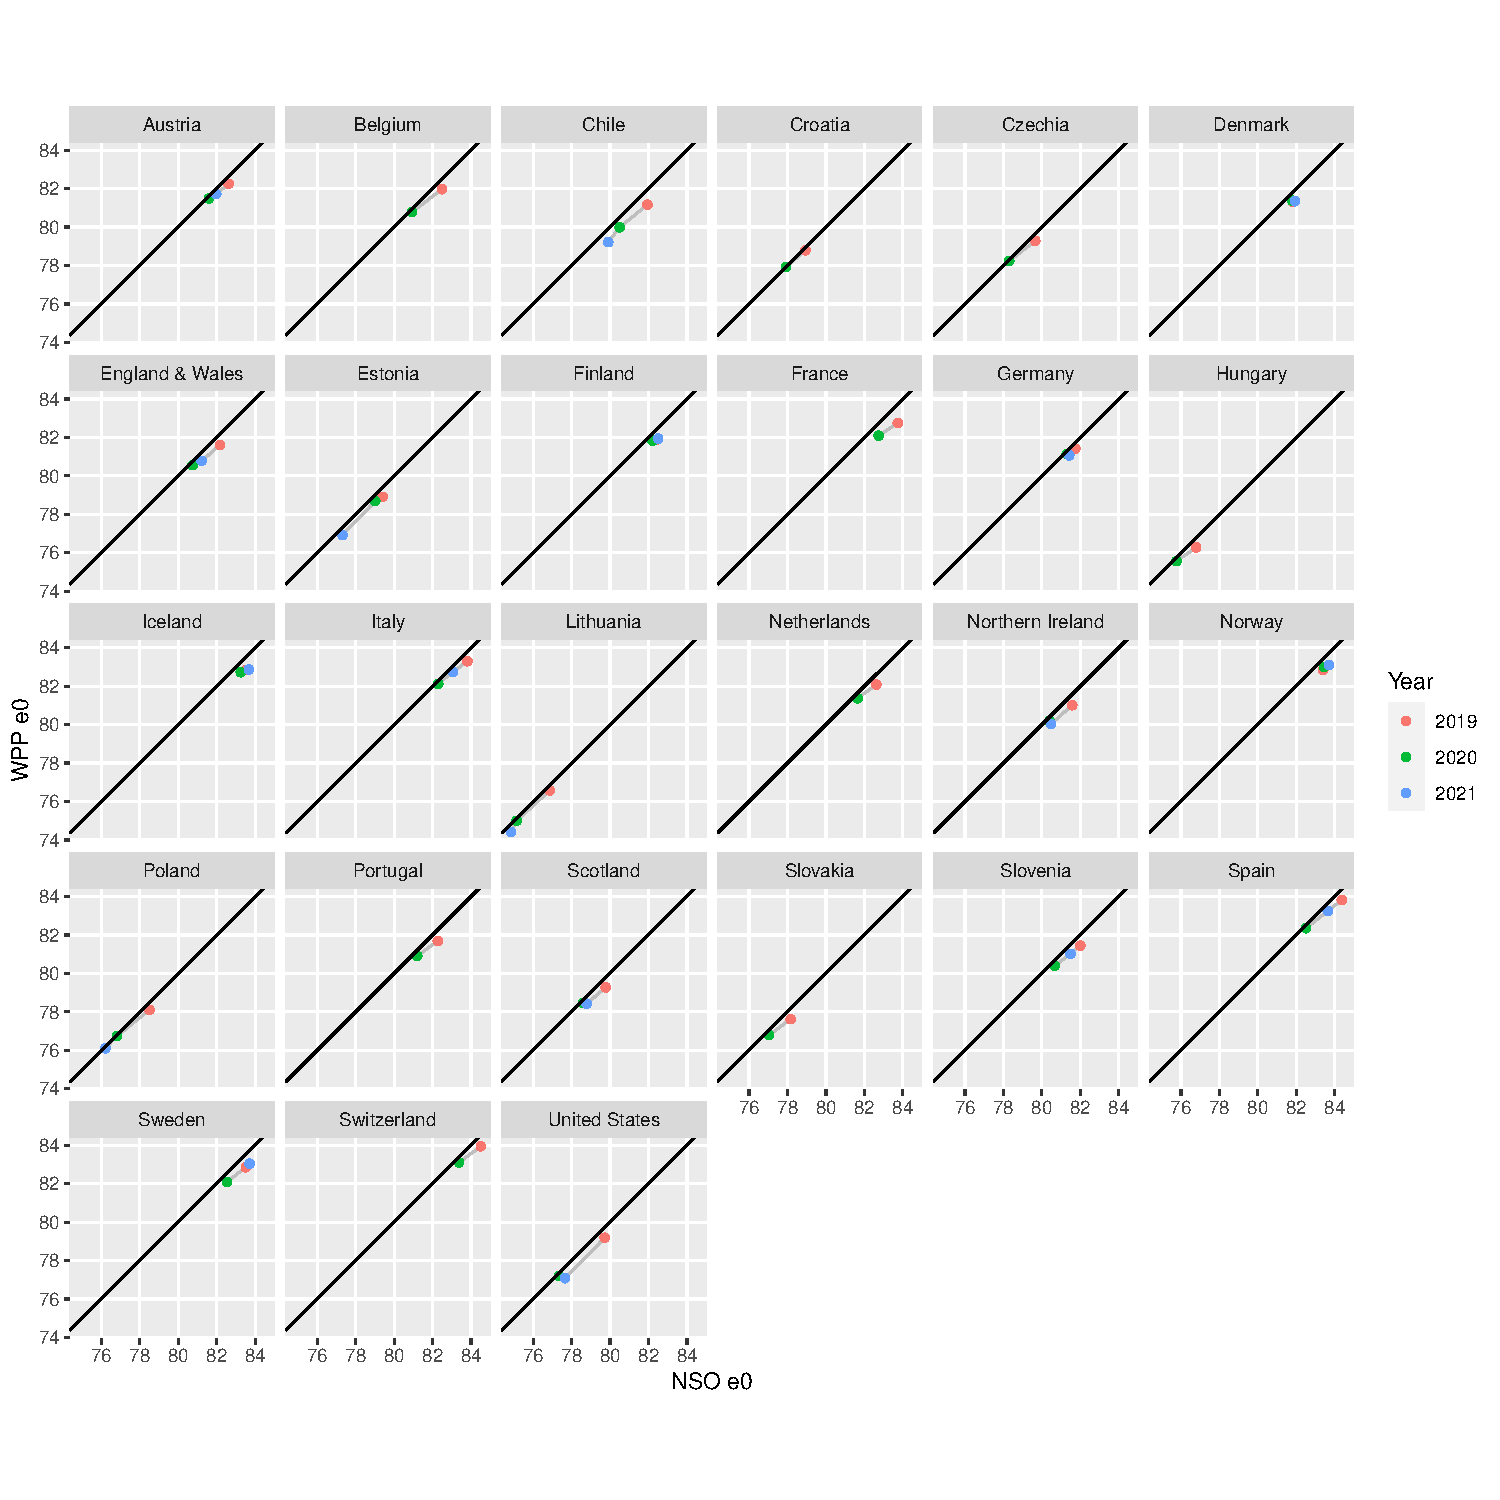
\includegraphics[width=\textwidth]{figure-s1.pdf}
    \caption{Life expectancy (e0) estimates for 2019, 2020 and when available 2021, using population estimates from national statistical offices (NSOs) (x-axis) and UN World Population Prospects (WPP) (y-axis). Black line indicates x=y line.}
    \label{fig:figure-a8}
\end{figure}

\end{document}
